\documentclass{standalone}
\usepackage{tikz}
\usetikzlibrary{patterns, positioning}

\begin{document}
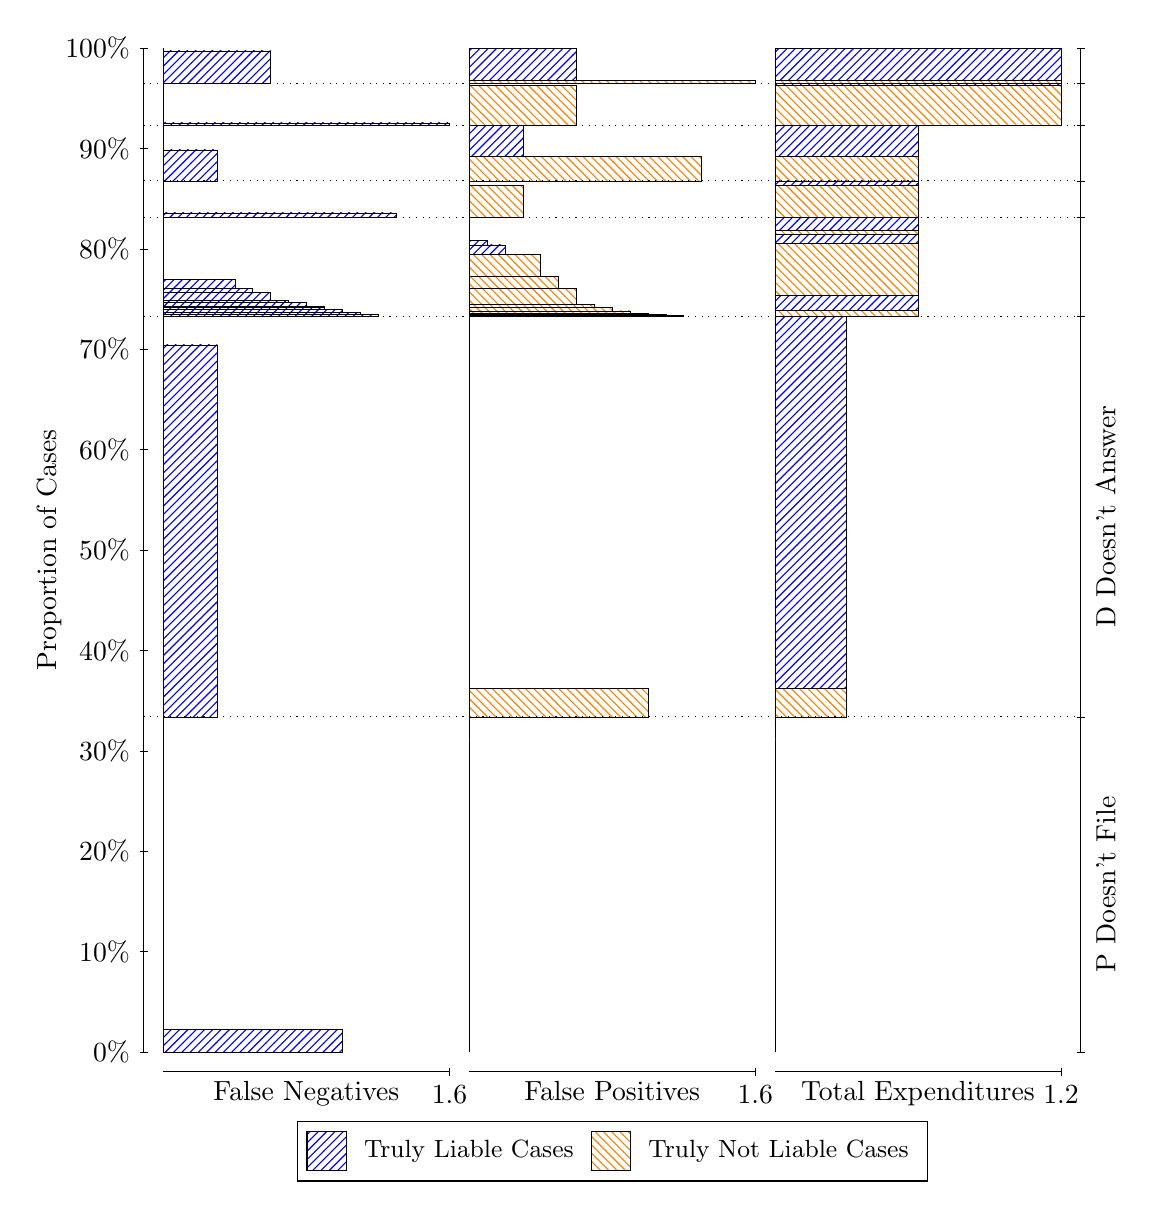
\begin{tikzpicture}
\draw[black, very thin] (1.5,1.75) -- (1.5,14.5);
\node[rotate=90, anchor=center] at (0.3, 8.125) {Proportion of Cases};
\draw[black, very thin] (1.45,1.75) -- (1.55,1.75);
\node[anchor=east] at (1.45, 1.75) {0\%};
\draw[black, very thin] (1.45,3.025) -- (1.55,3.025);
\node[anchor=east] at (1.45, 3.025) {10\%};
\draw[black, very thin] (1.45,4.3) -- (1.55,4.3);
\node[anchor=east] at (1.45, 4.3) {20\%};
\draw[black, very thin] (1.45,5.575) -- (1.55,5.575);
\node[anchor=east] at (1.45, 5.575) {30\%};
\draw[black, very thin] (1.45,6.85) -- (1.55,6.85);
\node[anchor=east] at (1.45, 6.85) {40\%};
\draw[black, very thin] (1.45,8.125) -- (1.55,8.125);
\node[anchor=east] at (1.45, 8.125) {50\%};
\draw[black, very thin] (1.45,9.4) -- (1.55,9.4);
\node[anchor=east] at (1.45, 9.4) {60\%};
\draw[black, very thin] (1.45,10.675) -- (1.55,10.675);
\node[anchor=east] at (1.45, 10.675) {70\%};
\draw[black, very thin] (1.45,11.95) -- (1.55,11.95);
\node[anchor=east] at (1.45, 11.95) {80\%};
\draw[black, very thin] (1.45,13.225) -- (1.55,13.225);
\node[anchor=east] at (1.45, 13.225) {90\%};
\draw[black, very thin] (1.45,14.5) -- (1.55,14.5);
\node[anchor=east] at (1.45, 14.5) {100\%};

\draw[black, very thin] (13.4,1.75) -- (13.4,14.5);
\draw[black, very thin] (13.35,1.75) -- (13.45,1.75);
\node[anchor=west] at (13.35, 1.75) {};
\draw[black, very thin] (13.35,6.0059) -- (13.45,6.0059);
\node[anchor=west] at (13.35, 6.0059) {};
\draw[black, very thin] (13.35,11.093) -- (13.45,11.093);
\node[anchor=west] at (13.35, 11.093) {};
\draw[black, very thin] (13.35,12.352) -- (13.45,12.352);
\node[anchor=west] at (13.35, 12.352) {};
\draw[black, very thin] (13.35,12.813) -- (13.45,12.813);
\node[anchor=west] at (13.35, 12.813) {};
\draw[black, very thin] (13.35,13.519) -- (13.45,13.519);
\node[anchor=west] at (13.35, 13.519) {};
\draw[black, very thin] (13.35,14.051) -- (13.45,14.051);
\node[anchor=west] at (13.35, 14.051) {};
\draw[black, very thin] (13.35,14.5) -- (13.45,14.5);
\node[anchor=west] at (13.35, 14.5) {};

\draw[black, very thin, pattern color=blue, pattern=north east lines] (1.75,1.75) rectangle (4.0208,2.0386);
\draw[black, very thin, pattern color=orange, pattern=north west lines] (1.75,2.0386) rectangle (1.75,6.0059);
\draw[black, very thin, pattern color=blue, pattern=north east lines] (1.75,6.0059) rectangle (2.4312,10.73);
\draw[black, very thin, pattern color=orange, pattern=north west lines] (1.75,10.73) rectangle (1.75,11.093);
\draw[black, very thin, pattern color=blue, pattern=north east lines] (1.75,11.093) rectangle (4.475,11.119);
\draw[black, very thin, pattern color=blue, pattern=north east lines] (1.75,11.119) rectangle (4.2479,11.144);
\draw[black, very thin, pattern color=blue, pattern=north east lines] (1.75,11.144) rectangle (4.0208,11.183);
\draw[black, very thin, pattern color=blue, pattern=north east lines] (1.75,11.183) rectangle (3.7937,11.208);
\draw[black, very thin, pattern color=blue, pattern=north east lines] (1.75,11.208) rectangle (3.7937,11.223);
\draw[black, very thin, pattern color=blue, pattern=north east lines] (1.75,11.223) rectangle (3.5667,11.27);
\draw[black, very thin, pattern color=blue, pattern=north east lines] (1.75,11.27) rectangle (3.3396,11.297);
\draw[black, very thin, pattern color=blue, pattern=north east lines] (1.75,11.297) rectangle (3.1125,11.392);
\draw[black, very thin, pattern color=blue, pattern=north east lines] (1.75,11.392) rectangle (2.8854,11.445);
\draw[black, very thin, pattern color=blue, pattern=north east lines] (1.75,11.445) rectangle (2.6583,11.566);
\draw[black, very thin, pattern color=orange, pattern=north west lines] (1.75,11.566) rectangle (1.75,12.352);
\draw[black, very thin, pattern color=blue, pattern=north east lines] (1.75,12.352) rectangle (4.7021,12.406);
\draw[black, very thin, pattern color=orange, pattern=north west lines] (1.75,12.406) rectangle (1.75,12.813);
\draw[black, very thin, pattern color=blue, pattern=north east lines] (1.75,12.813) rectangle (2.4312,13.206);
\draw[black, very thin, pattern color=orange, pattern=north west lines] (1.75,13.206) rectangle (1.75,13.519);
\draw[black, very thin, pattern color=blue, pattern=north east lines] (1.75,13.519) rectangle (5.3833,13.549);
\draw[black, very thin, pattern color=orange, pattern=north west lines] (1.75,13.549) rectangle (1.75,14.051);
\draw[black, very thin, pattern color=blue, pattern=north east lines] (1.75,14.051) rectangle (3.1125,14.465);
\draw[black, very thin, pattern color=orange, pattern=north west lines] (1.75,14.465) rectangle (1.75,14.5);
\draw[black, very thin, pattern color=orange, pattern=north west lines] (5.6333,1.75) rectangle (5.6333,5.7173);
\draw[black, very thin, pattern color=blue, pattern=north east lines] (5.6333,5.7173) rectangle (5.6333,6.0059);
\draw[black, very thin, pattern color=orange, pattern=north west lines] (5.6333,6.0059) rectangle (7.9042,6.3692);
\draw[black, very thin, pattern color=blue, pattern=north east lines] (5.6333,6.3692) rectangle (5.6333,11.093);
\draw[black, very thin, pattern color=orange, pattern=north west lines] (5.6333,11.093) rectangle (8.3583,11.103);
\draw[black, very thin, pattern color=orange, pattern=north west lines] (5.6333,11.103) rectangle (8.1313,11.113);
\draw[black, very thin, pattern color=orange, pattern=north west lines] (5.6333,11.113) rectangle (7.9042,11.134);
\draw[black, very thin, pattern color=orange, pattern=north west lines] (5.6333,11.134) rectangle (7.6771,11.161);
\draw[black, very thin, pattern color=orange, pattern=north west lines] (5.6333,11.161) rectangle (7.45,11.205);
\draw[black, very thin, pattern color=orange, pattern=north west lines] (5.6333,11.205) rectangle (7.2229,11.24);
\draw[black, very thin, pattern color=orange, pattern=north west lines] (5.6333,11.24) rectangle (6.9958,11.451);
\draw[black, very thin, pattern color=orange, pattern=north west lines] (5.6333,11.451) rectangle (6.7687,11.599);
\draw[black, very thin, pattern color=orange, pattern=north west lines] (5.6333,11.599) rectangle (6.5417,11.879);
\draw[black, very thin, pattern color=blue, pattern=north east lines] (5.6333,11.879) rectangle (6.0875,12.001);
\draw[black, very thin, pattern color=blue, pattern=north east lines] (5.6333,12.001) rectangle (5.8604,12.054);
\draw[black, very thin, pattern color=blue, pattern=north east lines] (5.6333,12.054) rectangle (5.6333,12.352);
\draw[black, very thin, pattern color=orange, pattern=north west lines] (5.6333,12.352) rectangle (6.3146,12.76);
\draw[black, very thin, pattern color=blue, pattern=north east lines] (5.6333,12.76) rectangle (5.6333,12.813);
\draw[black, very thin, pattern color=orange, pattern=north west lines] (5.6333,12.813) rectangle (8.5854,13.127);
\draw[black, very thin, pattern color=blue, pattern=north east lines] (5.6333,13.127) rectangle (6.3146,13.519);
\draw[black, very thin, pattern color=orange, pattern=north west lines] (5.6333,13.519) rectangle (6.9958,14.021);
\draw[black, very thin, pattern color=blue, pattern=north east lines] (5.6333,14.021) rectangle (5.6333,14.051);
\draw[black, very thin, pattern color=orange, pattern=north west lines] (5.6333,14.051) rectangle (9.2667,14.087);
\draw[black, very thin, pattern color=blue, pattern=north east lines] (5.6333,14.087) rectangle (6.9958,14.5);
\draw[black, very thin, pattern color=orange, pattern=north west lines] (9.5167,1.75) rectangle (9.5167,5.7173);
\draw[black, very thin, pattern color=blue, pattern=north east lines] (9.5167,5.7173) rectangle (9.5167,6.0059);
\draw[black, very thin, pattern color=orange, pattern=north west lines] (9.5167,6.0059) rectangle (10.425,6.3692);
\draw[black, very thin, pattern color=blue, pattern=north east lines] (9.5167,6.3692) rectangle (10.425,11.093);
\draw[black, very thin, pattern color=orange, pattern=north west lines] (9.5167,11.093) rectangle (11.333,11.168);
\draw[black, very thin, pattern color=blue, pattern=north east lines] (9.5167,11.168) rectangle (11.333,11.363);
\draw[black, very thin, pattern color=orange, pattern=north west lines] (9.5167,11.363) rectangle (11.333,12.019);
\draw[black, very thin, pattern color=blue, pattern=north east lines] (9.5167,12.019) rectangle (11.333,12.134);
\draw[black, very thin, pattern color=orange, pattern=north west lines] (9.5167,12.134) rectangle (11.333,12.189);
\draw[black, very thin, pattern color=blue, pattern=north east lines] (9.5167,12.189) rectangle (11.333,12.352);
\draw[black, very thin, pattern color=orange, pattern=north west lines] (9.5167,12.352) rectangle (11.333,12.76);
\draw[black, very thin, pattern color=blue, pattern=north east lines] (9.5167,12.76) rectangle (11.333,12.813);
\draw[black, very thin, pattern color=orange, pattern=north west lines] (9.5167,12.813) rectangle (11.333,13.127);
\draw[black, very thin, pattern color=blue, pattern=north east lines] (9.5167,13.127) rectangle (11.333,13.519);
\draw[black, very thin, pattern color=orange, pattern=north west lines] (9.5167,13.519) rectangle (13.15,14.021);
\draw[black, very thin, pattern color=blue, pattern=north east lines] (9.5167,14.021) rectangle (13.15,14.051);
\draw[black, very thin, pattern color=orange, pattern=north west lines] (9.5167,14.051) rectangle (13.15,14.087);
\draw[black, very thin, pattern color=blue, pattern=north east lines] (9.5167,14.087) rectangle (13.15,14.5);
\draw[black, dotted] (1.5,6.0059) -- (13.4,6.0059);
\draw[black, dotted] (1.5,11.093) -- (13.4,11.093);
\draw[black, dotted] (1.5,12.352) -- (13.4,12.352);
\draw[black, dotted] (1.5,12.813) -- (13.4,12.813);
\draw[black, dotted] (1.5,13.519) -- (13.4,13.519);
\draw[black, dotted] (1.5,14.051) -- (13.4,14.051);
\draw[black, very thin] (1.75,1.5) -- (5.3833,1.5);
\node[anchor=north] at (3.5667, 1.5) {False Negatives};
\draw[black, very thin] (5.3833,1.45) -- (5.3833,1.55);
\node[anchor=north] at (5.3833, 1.45) {1.6};

\draw[black, very thin] (5.6333,1.5) -- (9.2667,1.5);
\node[anchor=north] at (7.45, 1.5) {False Positives};
\draw[black, very thin] (9.2667,1.45) -- (9.2667,1.55);
\node[anchor=north] at (9.2667, 1.45) {1.6};

\draw[black, very thin] (9.5167,1.5) -- (13.15,1.5);
\node[anchor=north] at (11.333, 1.5) {Total Expenditures};
\draw[black, very thin] (13.15,1.45) -- (13.15,1.55);
\node[anchor=north] at (13.15, 1.45) {1.2};

\node[black, centered, rotate=90] at (13.72, 3.8779) {P Doesn't File};
\node[black, centered, rotate=90] at (13.72, 8.5496) {D Doesn't Answer};






\draw (7.449999999999999,1.5) node[draw=none] (baseCoordinate) {};
\begin{scope}[align=center]
        \matrix[scale=0.5, draw=black, below=0.5cm of baseCoordinate, nodes={draw}, column sep=0.1cm]{
            \node[rectangle, draw, minimum width=0.5cm, minimum height=0.5cm, pattern=north east lines, pattern color=blue] {}; &
            \node[draw=none, font=\small] (B) {Truly Liable Cases}; &
            \node[rectangle, draw, minimum width=0.5cm, minimum height=0.5cm, pattern=north west lines, pattern color=orange] {}; &
            \node[draw=none, font=\small] (B) {Truly Not Liable Cases}; \\
            };
\end{scope}

\end{tikzpicture}
\end{document}